\chapter{Introducción}
Este proyecto es software libre, y está publicado con la licencia \cite{gplv3} General Public License v3

\section{Motivación} 
El tratamiento automático de la información por medio de técnicas matemáticas procesadas por un ordenador ha cambiado la forma en la 
que nos organizabamos, estudiabamos y obteníamos conclusiones. La informática mejora la vida de las personas en númerosos campos, 
desde el entretenimiento personal a la mejora de la calidad en el sistema sanitario.

Numerosos estudios sociológicos avalan que la sanidad es una preocupación incesante de los españoles. Más acentuada si cabe recientemente
con la pandemia que sigue sufriendo el mundo.
\begin{figure}[]
	\centering	
	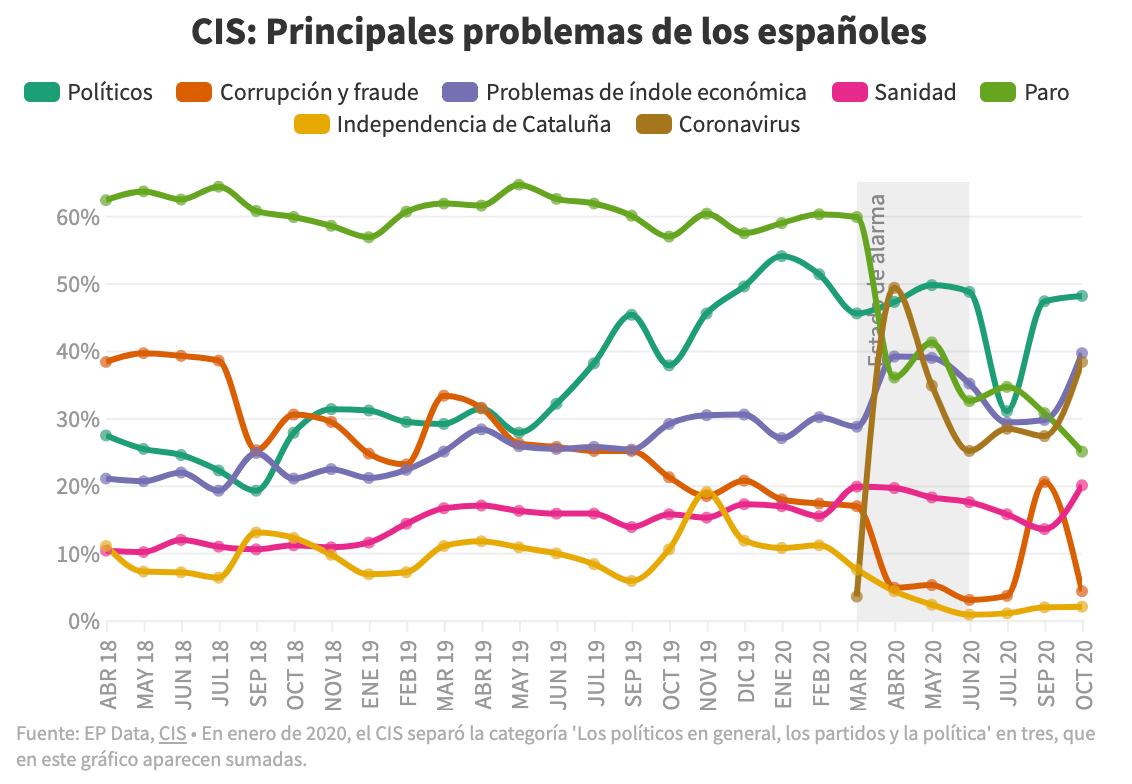
\includegraphics[scale=0.5]{logos/imgs/CIS_1.png}
	\caption{ \cite{rtve-cis}  Principales problemas de los españoles según el CIS }
    \label{fig:worst_f_value}
\end{figure}

La sanidad a pesar no estar exenta de movimientos sinusoidales en la preocupación de los españoles
siempre se muestra con una tendencia al alta solo superada por el paro y problemas de índole económico. 
Es evidente que la mejora del sistema sanitario es algo que nos concierne y repercute directamente en todos nosotros.

La ideación de un sistema capaz de realizar predicciones y visualizaciones con los datos públicos de las defunciones según 
la causa de muerte publicadas por el INE puede suponer una pequeña mejora del Sistema Nacional de Salud en materia de 
prevención de la enfermedad y promoción de la salud. Es necesario que el SNS sea capaz de realizar cribados preventivos 
más inteligentes mediante el conocimiento de la evolución de las causas de fallecimiento de los españoles.


\section{Objetivos}
El principal objetivo de este Trabajo Fin de Grado consiste en obtener un sistema de análisis de datos que nos aporte
información enriquecida sobre los datos publicados por el instituto nacional de estadística sobre las causas de muerte. 
Para conseguir el resultado final esperado debemos cumplir los siguientes objetivos:
\begin{itemize}
    \item Desarrollo de un modelo de datos que se adapte a los datos ofrecidos por el INE.
    \item Diseño y creción de una interfaz de programación de aplicaciones que ofrezca los datos procesados y 
filtrados a petición de usuarios o aplicaciones de terceros.
    \item Proveer de un punto de acceso visual para obtener gráficas y predicciones sobre los datos.
\end{itemize}

Una vez finalizado todo el proceso, además de haber obtenido la posibilidad de obtener la información 
desde un punto de acceso. Abrimos la posibilidad a usuarios experimentados de poder usar esta API para 
integrarla en sus soluciones o publicar los datos en los distintos formatos que nuestra API ofrece 
siempre que se mantenga la licencia original de publicación.

